\cleardoublepage
\chapter{Developed Architectures}

%%%%%%%%%%%%%%%%%%%%%%%%%%%%%%%%%%%%%%%%%%%%%%%%%%%%%%%%%%%%%%%%%%%%%%%%%%%%%%
\section{Software Implementations}

The previous chapter presented some characteristics of the current state of \emph{libaom}'s \emph{Transform} stage which might compromise its performance, the most relevant being the unnecessary flexibility in the representation of cosine approximations.

In order to undertake these opportunities, and improve the overall encoder performance, new architectures for the studied stage were developed. The first approach was to study possible simplifications of the reference software, through the development and testing of alternative approaches for the provided functions.

The developed implementations tackled the forward \emph{DCT}, since it was the \emph{kernel} that would have the most impact on encoder performance. As the \emph{IDCT} is shared between encoder and decoder, and due to the added complexity, no changes were done to this block, as it acts with accordance with the established standard, as mentioned previously. 

%%%%%%%%%%%%%%%%%%%%%%%%%%%%%%%%%%%%%%%
\subsection{Matrix Multiplication Implementation}

The first test was the application of the simplest integer \emph{DCT}, done by the multiplication of the input vector by a scaled up version of the transform matrix, $\mathbf{F}$, firstly shown in Equation \ref{eq:DCT2}. 

The original integer transform matrix is shown in Equation \ref{eq:matscale}.

\begin{equation} \label{eq:matscale}
    \begin{gathered}
        \mathbf{F}_{x,u} = \beta(u)\cos\left(\frac{(2x+1)u\pi }{2L}\right)\,0\leq u,x < L \\
        \Downarrow \\
        \mathbf{F} = \sqrt{\frac{2}{L}}  \begin{bmatrix}
            \sqrt{\frac{1}{2}}                                  & \sqrt{\frac{1}{2}}                                & \dots & \sqrt{\frac{1}{2}} \\
            \cos\left(\frac{\pi}{2L}\right)    & \cos\left(\frac{3\pi}{2L}\right) & \dots & \cos\left(\frac{(2(L-1)+1)\pi}{2L}\right) \\
            \vdots     & \vdots     & \ddots & \vdots       \\
            \cos\left(\frac{(L-1)\pi}{2L}\right)    & \cos\left(\frac{3(L-1)\pi}{2L}\right) & \dots & \cos\left(\frac{(2(L-1)+1)(L-1)\pi}{2L}\right) \\
        \end{bmatrix} 
    \end{gathered}
\end{equation}

As mentioned previously, the floating point coefficients bring a number of disadvantages on an hardware implementation, from increased calculation overheads, to encoder/decoder mismatches. 

In order to address these problems, a scale and rounding operation was performed, as shown in Equation \ref{eq:matscale}, where $K$ represents the number of bits of the scaled coefficients.

\begin{equation} \label{eq:matscale}
    \nint*{\mathbf{F}_K}   = \nint*{2^K \mathbf{F}}
\end{equation}

However, due to the rectangular block sizes allowed in \emph{AV1}, the factor $\sqrt{\nicefrac{2}{L}}$ isn't considered in the kernels themselves. Instead, the transformed outputs get scaled at a later stage. This way, the implemented transform matrix is

\begin{equation} \label{eq:matscale2}
    \begin{gathered}
        \nint*{\mathbf{F}_K}   = \nint*{2^K \sqrt{\frac{L}{2}}\mathbf{F}} \\
        = \nint*{2^K \begin{bmatrix}
                        \sqrt{\frac{1}{2}}                                  & \sqrt{\frac{1}{2}}                                & \dots & \sqrt{\frac{1}{2}} \\
                        \cos\left(\frac{\pi}{2L}\right)    & \cos\left(\frac{3\pi}{2L}\right) & \dots & \cos\left(\frac{(2(L-1)+1)\pi}{2L}\right) \\
                        \vdots     & \vdots     & \ddots & \vdots       \\
                        \cos\left(\frac{(L-1)\pi}{2L}\right)    & \cos\left(\frac{3(L-1)\pi}{2L}\right) & \dots & \cos\left(\frac{(2(L-1)+1)(L-1)\pi}{2L}\right) \\
                    \end{bmatrix} 
                }
    \end{gathered}
\end{equation}

This way, the  transformed outputs are calculated through

\begin{equation}
    \vec{\mathcal{G}} = \left[\nint*{\mathbf{F}_K} \vec{g}\right]>>K
\end{equation}

For an $L$ length vector, the calculation of the transformed vector implies $L^2$ additions and $L^2$ multiplications, which leads to the main disadvantage of such implementation. For larger vectors, this operation becomes too demanding in terms of memory and complexity.

One other negative aspect of such implementation is that, due to the variation of the transform matrix's coefficients, the obtained error in the rounding and scaling operation also varies with the vector size. The quantization\footnote{Here, quantization refers to the scaling and rounding operation, and not to the the \emph{Q} stage in an encoder.} error, $\Delta_K$, can be calculated as

\begin{equation}
    \Delta_K = \frac{\max{\left(\sqrt{\frac{L}{2}}\mathbf{F}\right)} - \min{\left(\sqrt{\frac{L}{2}}\mathbf{F}\right)}}{2^K}
\end{equation}

As it was proven in the previous Chapter that the number of bits in the cosine representation wouldn't greatly impact the quality of the video, the developed architectures used 8 bits for the scaling operation, as to decrease the overhead of the implemented multiplications and shifts. The impact of this choice was evaluated at a later stage.

To evaluate the performance of this first implementation, there was performed a test that measured and compared the elapsed time for both the described architecture, and the corresponding equivalent from \emph{aomenc}. This test injected a fixed sequence of input vectors into each of the \emph{DCT}'s, scaled the vectors in the same manner as the encoder, and then re-transformed the obtained vectors with \emph{AV1}'s \emph{IDCT}. This sequence of operations was timed, and the corresponding results are presented at Table \ref{tab:dcttime}.

\begin{table}[!htpb]
    \centering
    \begin{tabular}{ccc} \toprule
        \multirow{2}{*}{\textbf{Vector Size}} &     \multicolumn{2}{c}{\textbf{Execution Time (ms)}} \\
         &      \textbf{aomenc's} &      \textbf{MM} \\ \toprule
        \textbf{4} &    145 &      98 $(-32.5\%)$ \\ \hline
        \textbf{8} &    319 &      215 $(-32.6\%)$ \\ \hline
        \textbf{16} &   787 &      583 $(-25.9\%)$ \\ \hline
        \textbf{32} &   1917 &     1606 $(-16.2\%)$  \\ \hline
        \textbf{64} &   4999  &    5696 $(+14.0\%)$  \\ 
        \bottomrule
    \end{tabular}
    \caption{Comparison of execution time between \emph{aomenc}'s DCT and the matrix multiplication implementation.}
    \label{tab:dcttime}
\end{table}

From these results it's easily observable why the currently implemented transforms follow the \emph{butterfly} scheme. Although from sizes $4$ to $32$, the proposed implementation is faster than the current version of \emph{libaom}, the largest transform is slower. This factor, added to the error variation from the scaling operation makes this implementation quite damaging for the overall encoder performance, especially on a constant quality objective, as shown in Table \ref{tab:multresults}. Here, there are presented the timing results of an encoding test, where one encode was made with the standard \emph{aomenc}, the other had the proposed matrix multiplication \emph{DCT}'s. The test encoded the first 15 frames of the \emph{Parkrun} HD sequence, with two different quality objectives. After compression, the encoded video was decoded with \emph{aomdec}, calculating the PSNR of the output video.

\begin{table}[!htpb]
    \centering
    \begin{tabular}{cccc} \toprule
        \multirow{2}{*}{\textbf{cq-level}} & \multirow{2}{*}{\textbf{Measure}} &    \multicolumn{2}{c}{\textbf{Execution Time (ms)}} \\
        &   &   \textbf{Original} &      \textbf{MM} \\ \toprule
         \multirow{3}{*}{\textbf{60}}   & \textbf{Total time (s)}       & 466.5     & 530.8 \\
                                        & \textbf{\emph{Trans.} time (s)}    & 45.0      & 104.2 \\
                                        & \textbf{PSNR (dB)}            & 32.39     & 32.38 \\ \hline
         \multirow{3}{*}{\textbf{5}}    & \textbf{Total time (s)}       & 814.1     & 835.3 \\
                                        & \textbf{\emph{Trans.} time (s)}    & 60.4      & 98.4 \\
                                        & \textbf{PSNR (dB)}            & 34.88     & 34.86 \\                                        
         \bottomrule
    \end{tabular}
    \caption{\emph{aomenc}'s encoding time with original vs implemented \emph{DCT}.}
    \label{tab:multresults}
\end{table}

As it is observable, to maintain a similar encoding quality, the encoder spends up to $13.8\%$ more time per encode, making such architecture unreliable for implementation on \emph{aomenc}.

Taking this into account, a new approach was employed, using the same \emph{butterfly} scheme as \emph{libaom}'s transforms.

%%%%%%%%%%%%%%%%%%%%%%%%%%%%%%%%%%%%%%%
\subsection{Alternative \emph{Butterfly} Implementation}

\emph{AV1}'s reference \emph{Transform stage} follows the aforementioned architecture for the DCT, in addition to expanding its use into the \emph{ADST}. In the publishing work \cite{wen-hsiungchenFastComputationalAlgorithm1977}, the authors give good reasons for the heavy adoption of this implementation, claiming that "\emph{The number of computational steps has been shown to be less than \nicefrac{1}{6} of the conventional DCT algorithm employing a 2-sided FFT}". 

This is achieved through a pipelined implementation of the previously shown matrix multiplication, where each stage is calculated as function of the previously calculated intermediary coefficients, as shown in Chapter \ref{chap:trans}. Besides the reduction of complexity, this implementation also uses a fixed bank of \emph{cosine} coefficients (corresponding to \texttt{cospi} in \emph{libaom}), limited between $\cos\left(\nicefrac{\pi}{2}\right) \leq \alpha \leq \cos(0)$, i.e., $0 \leq \alpha \leq 1$. This way, the quantization error produced by the rounding and scaling operation is constant for all vector sizes.

To improve upon the reference \emph{DCT}, the developed architecture implemented a similar approach to the previous \emph{MM} architecture, using 8 bits for the scaling of the \emph{cosine} approximations. These values, $cos_{Apr}$ were generated using the same method as \texttt{cospi}, i.e.

\begin{equation}
    cos_{Apr} = \nint*{2^8*\cos\left(\frac{k\pi}{128}\right)}
\end{equation}

Comparing the quantization step to the worst case for \emph{libaom}'s \emph{DCT}, with 10 bits

\nocite{shiImageVideoCompression2008}

\begin{gather}
    \Delta_{10} = \frac{1-0}{2^{10}} \approx 0.98\cdot10^{-3}\\
    \Delta_{8} = \frac{1-0}{2^{8}} \approx 3.9\cdot10^{-3}
\end{gather}
then it's possible to calculate the \emph{Mean Squared Quantization Error} through Equation \ref{eq:msequant}

\begin{equation} \label{eq:msequant}
    \begin{gathered}
        MSE_{Kq} = \frac{\Delta_K^2}{12} \\
        \Downarrow \\
        MSE_{10q} \approx 79.5 \cdot 10^{-9} \\
        MSE_{8q} \approx 1271.6 \cdot 10^{-9} = 16\cdot MSE_{10q} 
    \end{gathered}
\end{equation}

Although this value might seem discouraging, most of the error introduced in this stage is irrelevant once considered the error created by the encoder's \emph{Quantization} block. With that said, the impact of this approximation might compromise the encoder on higher quality (i.e., lower \emph{Quantizer}) objectives.

The implemented \emph{DCT} also deviates from the reference software in the multiplication of the cosine coefficients. The latter version calculated most of the intermediary functions with the \texttt{half\_btf} function (Equation \ref{eq:half_btf}), which, because the additional $2^(K-1)$, performs a \emph{rounding} (\gls{tld:round}) operation as shown in Equation \ref{eq:alternhalfbtf}

\begin{equation} \label{eq:alternhalfbtf}
    \begin{gathered}
        \texttt{half\_btf(w0, in0, w1, in1, K)} \equiv \left(w_0\cdot in_0 + w_1\cdot in_1 + (1<<(K-1))\right)>>(K) \\
        \Downarrow \\
        \nint*{\frac{w_0\cdot in_0 + w_1\cdot in_1}{2^{K}}}
    \end{gathered}    
\end{equation}

On the implemented architecture, the rescaling didn't include the additional factor, and was made just with the right shifting (\gls{tld:shiftr}) by 8 bits, corresponding to the \emph{flooring} operation (\gls{tld:floor}).

The constructed \emph{DCT} architecture underwent the same test as the previous implementation, giving origin to the results from Table \ref{tab:dcttime2}.

\begin{table}[!htpb]
    \centering
    \begin{tabular}{ccc} \toprule
        \multirow{2}{*}{\textbf{Vector Size}} &     \multicolumn{2}{c}{\textbf{Execution Time (ms)}} \\
         &      \textbf{aomenc's} &      \textbf{Alternative \emph{butterfly}} \\ \toprule
        \textbf{4} &    142 &      97 $(-31.3\%)$ \\ \hline
        \textbf{8} &    326 &      229 $(-29.9\%)$ \\ \hline
        \textbf{16} &   785 &      544 $(-30.7\%)$ \\ \hline
        \textbf{32} &   1938 &     1320 $(-31.9\%)$  \\ \hline
        \textbf{64} &   4986  &    3562 $(-28.5\%)$  \\ 
        \bottomrule
    \end{tabular}
    \caption{Comparison of execution time between \emph{aomenc}'s DCT and the alternative \emph{butterfly} implementation.}
    \label{tab:dcttime2}
\end{table}

As shown, the developed architecture is approximately $30\%$ for all vector sizes. This is due to the removal of the memory accessing overheads imposed by the access to the \texttt{cospi} array, as well the simplification of the performed operations. 

However, the liability of this implementation depends on whether the encoder can maintain the desired quality with the increased error introduced by the quantization of the \emph{cosine} approximations. To verify this factor, the tests presented in Section \ref{ssec:performance} were repeated, once with the original encoder, and other with the encoder with the described alternative version of the \emph{DCT}. The obtained quality and timing results are presented in Figures \ref{fig:buttqual} and \ref{fig:butttime}. In the latter, the dotted lines correspond to time with the original encoder. The percentage above each bar represent the time difference taken by the alternative encoder, relative to the original.

\begin{figure}[!htpb]
    \centering
    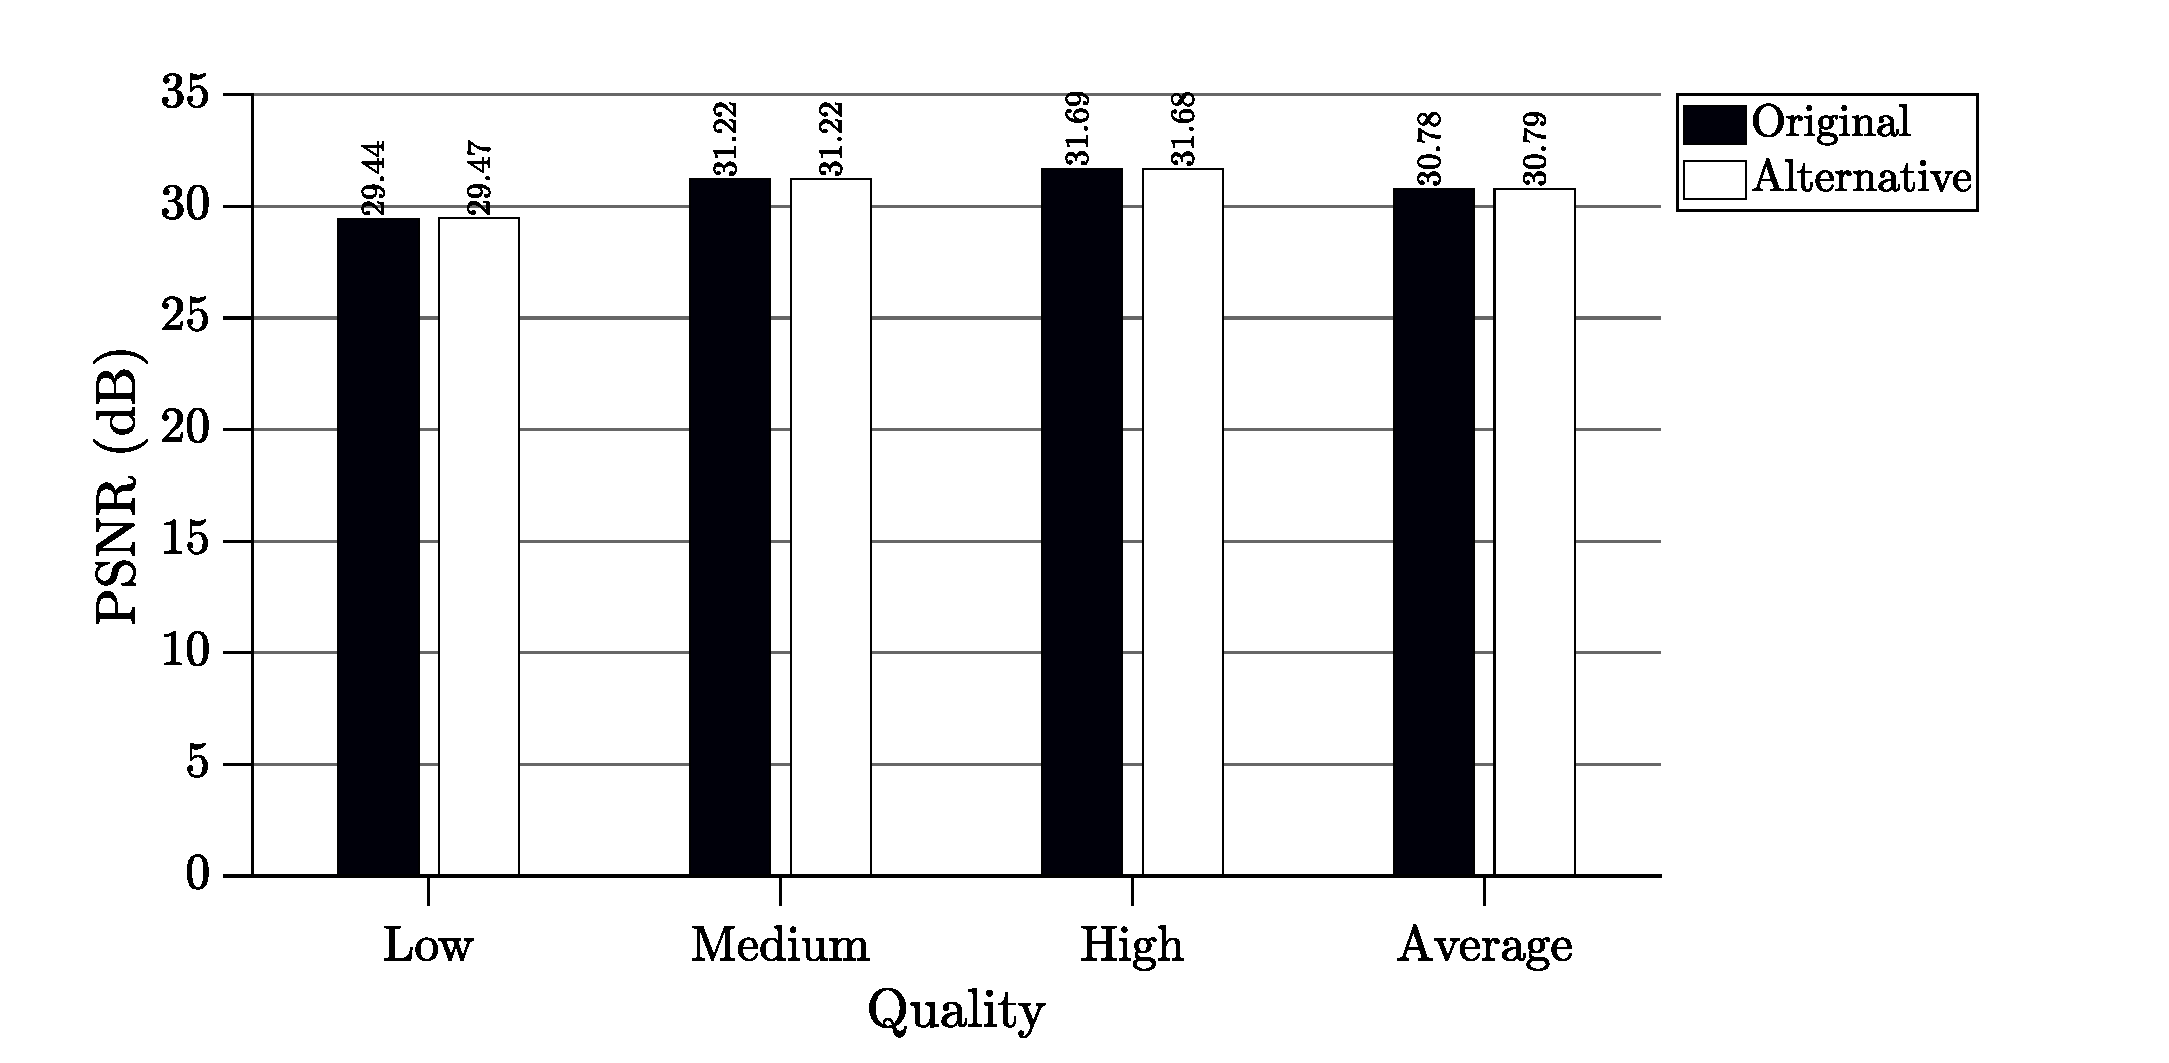
\includegraphics[width=\textwidth]{Sections/4DevelopedArchitecture/Figures/buttmultqual.eps}
    \caption{Obtained quality with original vs alternative \emph{DCT} implementation.}
    \label{fig:buttqual}
\end{figure}

\begin{figure}[!htpb]
    \centering
    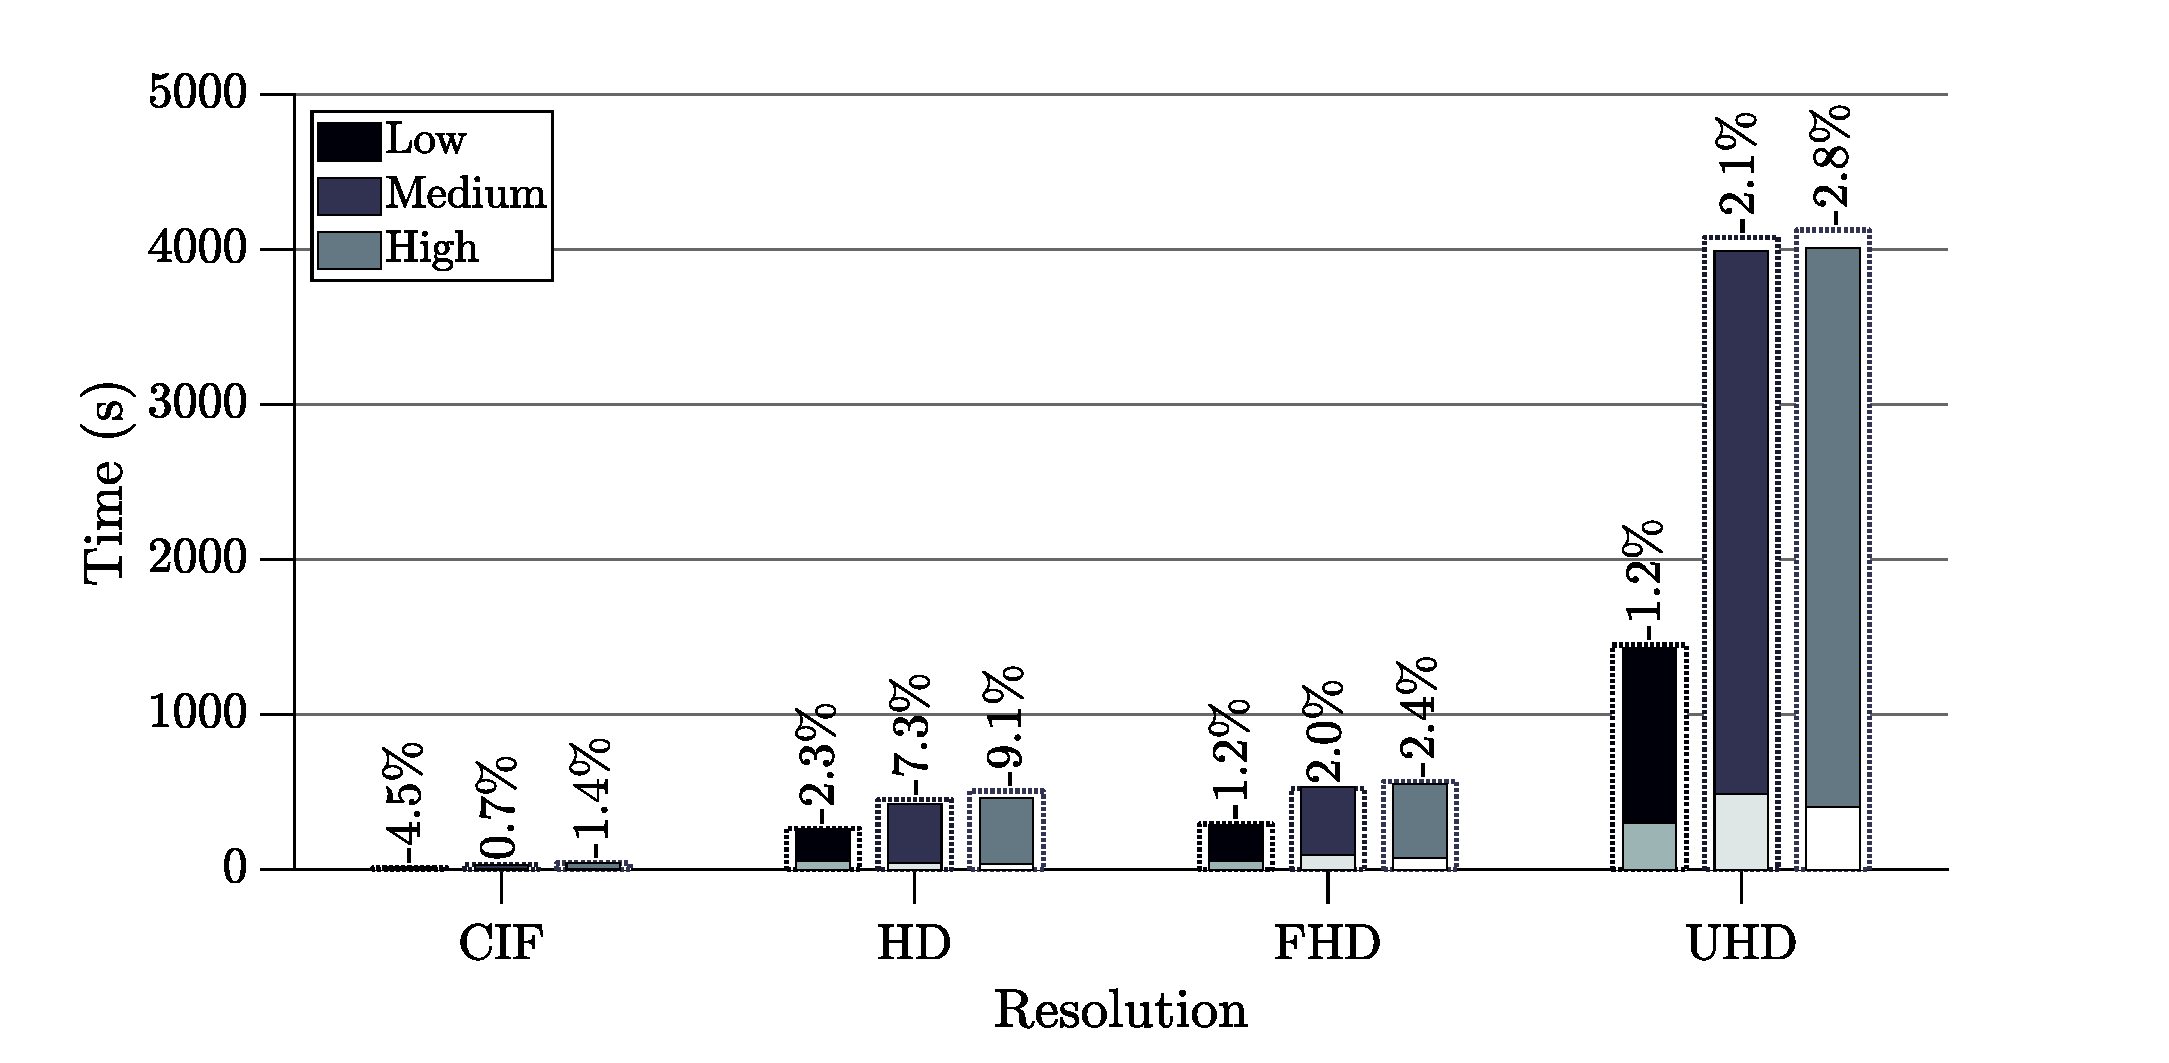
\includegraphics[width=\textwidth]{Sections/4DevelopedArchitecture/Figures/buttmulttime.eps}
    \caption{Encoding time with original vs alternative \emph{DCT} implementation.}
    \label{fig:butttime}
\end{figure}

As shown, with the performed changes, the encoding time was, in average, reduced for all quality objectives, while maintaining the output PSNR. These results allow to advance to an efficient hardware implementation, since the obtained architecture can heavily benefit from parallelization and, due to the discarding of the \texttt{cospi} array, would need less memory than the original architecture.

%%%%%%%%%%%%%%%%%%%%%%%%%%%%%%%%%%%%%%%%%%%%%%%%%%%%%%%%%%%%%%%%%%%%%%%%%%%%%%
\section{Parallel Hardware Implementation}

\clearpage
\printbibliography[heading=subbibliography]
\addcontentsline{toc}{section}{References}